\chapter{Implementation} \label{C:implementation} 
This chapter discusses the details of the Kihi implementation presented in this report. The heart of this chapter is a description of the various performance driven designs decisions and features made and developed for this implementation of Kihi. However, in order to understand that an understanding of the basic implementation is necessary. Specifically, how the semantics outlined in chapter \ref{C:background} can be implemented as code. But firstly, in order to guide the rest of the chapter, an overview of the implementation is presented below.

\section{Overview}
The executable implemented in this project is capable of executing Kihi source directly. Internally, the source code is first parsed and transformed into an intermediary representation before execution. The details of the intermediary representation are discussed in section \ref{sec:implementation_intermediary_representation}. The execution process involves selecting an executor, which can be understood as a virtual machine, and utilising it to execute the intermediary representation. The executable supports three types of executors: a term rewriting based executor, a stack based executor, and a depreciated term rewriting based executor kept for posterity. The implementation details of these executors are provided in section \ref{sec:implementation_executors}

The implementation provides various configuration options available at compile time and run time. Compile time options are available through feature flags and run time options can be specified with command line flags. Feature flags make it possible to include or exclude various features such as the aforementioned executors, CPU profiling, and output printing. The run time arguments make it possible to specify which executor to utilise, degree of optimisation and number of outputs to print. More specific details are available in the project's readme.

\todo[inline]{
    maybe in background elaborate on what a virtual machine is?
}

\todo[inline]{
    move this:
    This intermediary representation is mostly identical to the grammar shown in figure \ref{fig:kihi_grammar} barring implementation details, debugging symbols, and optimisation mechanisms. The optimisation mechanisms are of particular interest and are discussed in greater detail in section \ref{sec:implementation_optimisation}.
    The executable takes as an argument the path to a text file contain Kihi source code, encoded in either UTF-8 or ASCII, and subsequently runs the program, emitting any outputs to standard output.
}

\section{Implementation Language}
This project was implemented in Rust. This decision was largely motivated by performance concerns and ease of use. Rust is considered a systems language and is designed with performance as a principal goal. An manifestation of this is manual control over memory in conjunction with a type system capable of guaranteeing memory safety. This provides the performance benefits of a low level language while retaining the safety benefits of a garbage collected language. Furthermore, Rust also provides many features commonly found in functional programming languages, such as pattern matching, which significantly improve the ergonomics of the language especially in the context of programming language implementation as shown by the ubiquitous of such features throughout the codebase. Overall, these factors give Rust well earned respect as a language suitable for performance sensitive projects, and an especially compelling choice for this project.

\todo[inline]{Reference rust webpage?}

\section{Intermediary Representation}\label{sec:implementation_intermediary_representation}
The intermediary representation is mostly identical to the grammar shown in figure \ref{fig:kihi_grammar} barring implementation details, debugging symbols, and optimisation mechanisms. The purpose of the intermediary representation is two fold. Firstly, it decouples the source code from the executable representation allowing room for interpretation and optimisations. Secondly, it provides a common representation that can be interpreted by the various executors. Figure \ref{fig:kihi_intermediary_representation} shows the

\tikzstyle{startstop} = [rectangle, rounded corners, minimum width=3cm, minimum height=1cm,text centered, draw=black, fill=red!30]
\tikzstyle{io} = [trapezium, trapezium left angle=70, trapezium right angle=110, minimum width=3cm, minimum height=1cm, text centered, draw=black, fill=blue!30]
\tikzstyle{process} = [rectangle, minimum width=3cm, minimum height=1cm, text centered, draw=black, fill=orange!30]
\tikzstyle{decision} = [diamond, minimum width=3cm, minimum height=1cm, text centered, draw=black, fill=green!30]
\tikzstyle{arrow} = [thick,->,>=stealth]

\tikzstyle{plain_box} = [rectangle, minimum width=5cm, minimum height=1.2cm, text width=4cm, text centered, draw=black]
\begin{figure}[htb]
    \centering
    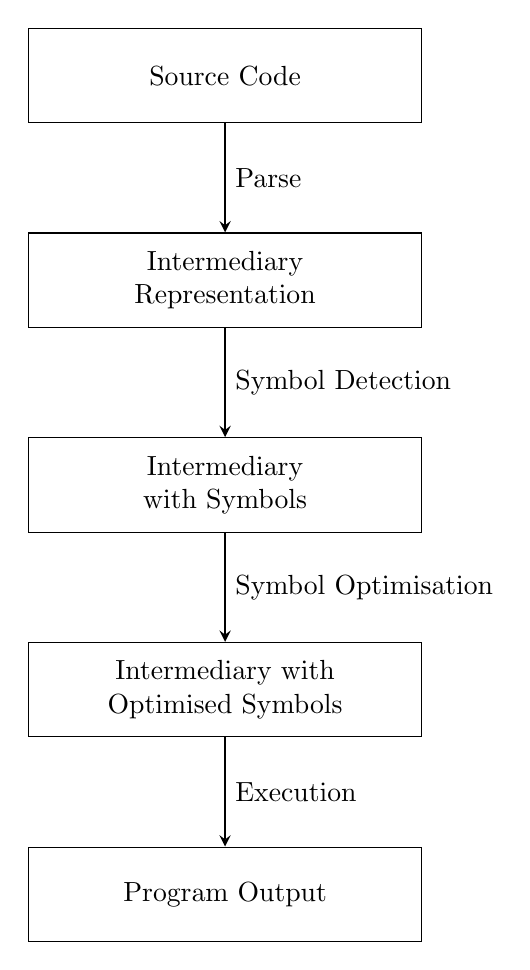
\begin{tikzpicture}[node distance=2.6cm]
        \node (source) [plain_box] {Source Code};
        \node (intermediary) [plain_box, below of=source] {Intermediary Representation};
        \node (intermediary_1) [plain_box, below of=intermediary] {Intermediary with Symbols};
        \node (intermediary_2) [plain_box, below of=intermediary_1] {Intermediary with Optimised Symbols};
        \node (execution) [plain_box, below of=intermediary_2] {Program Output};

        \draw [arrow] (source) -- node[anchor=west] {Parse} (intermediary);
        \draw [arrow] (intermediary) -- node[anchor=west] {Symbol Detection} (intermediary_1);
        \draw [arrow] (intermediary_1) -- node[anchor=west] {Symbol Optimisation} (intermediary_2);
        \draw [arrow] (intermediary_2) -- node[anchor=west] {Execution} (execution);
    \end{tikzpicture}
    \caption{How a Kihi program is executed.}
    \label{fig:kihi_execution_process}
\end{figure}
\tikzstyle{arrow} = [thick,->,>=stealth]

\tikzstyle{program} = [rectangle, minimum width=2.8cm, minimum height=1cm, text centered, node contents=Program, draw=black]

\tikzstyle{abstraction} = [rectangle, minimum width=2.8cm, minimum height=1cm, text centered, node contents=Abstraction, draw=black]

\tikzstyle{apply} = [rectangle, minimum width=2.8cm, minimum height=1cm, text centered, node contents=Apply, draw=black]

\tikzstyle{left} = [rectangle, minimum width=2.8cm, minimum height=1cm, text centered, node contents=Left, draw=black]

\tikzstyle{right} = [rectangle, minimum width=2.8cm, minimum height=1cm, text centered, node contents=Right, draw=black]

\tikzstyle{copy} = [rectangle, minimum width=2.8cm, minimum height=1cm, text centered, node contents=Copy, draw=black]

\tikzstyle{drop} = [rectangle, minimum width=2.8cm, minimum height=1cm, text centered, node contents=Drop, draw=black]

\begin{figure}[htb]
    \centering
    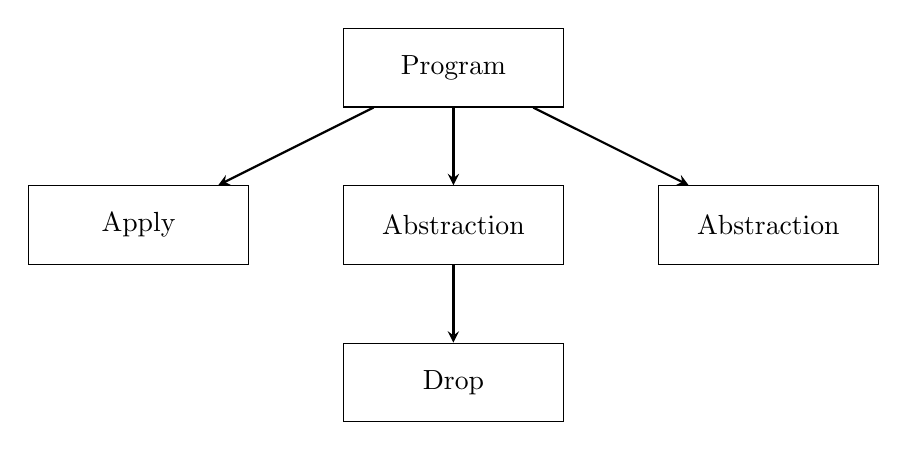
\begin{tikzpicture}[node distance=2cm]
        \node (program) [program];
        \node (2) [abstraction, below of=program];
        \node (1) [apply, left of=2, xshift=-2cm];
        \node (3) [abstraction, right of=2, xshift=2cm];
        \node (4) [drop, below of=2];

        \draw [arrow] (program) -- (1);
        \draw [arrow] (program) -- (2);
        \draw [arrow] (program) -- (3);
        \draw [arrow] (2) -- (4);
    \end{tikzpicture}
    \caption{Kihi intermediary representation of the program: \lstinline{apply (drop) ()}}
    \label{fig:kihi_intermediary_representation_example_1}
\end{figure}


% · → × → (· · ← (→ → (·) ×)) (· ← (· · ← ← ()) × → (· · ← (·) · ← ← () · ← (×)) · ← ← ()) (↓)
\tikzstyle{symbol} = [rectangle, minimum width=2.8cm, minimum height=1cm, text centered, draw=black]

\begin{figure}[htb]
    \centering
    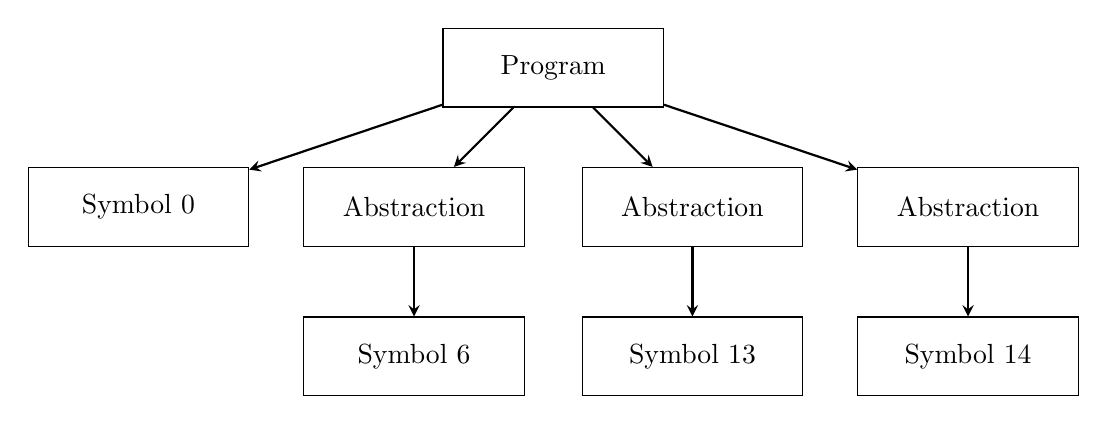
\begin{tikzpicture}[node distance=2.5cm]
        \node (program) [program];
        \node (2) [abstraction, below left of=program];
        \node (3) [abstraction, below right of=program];
        \node (1) [symbol, left of=2, xshift=-1cm] {Symbol 0};
        \node (4) [abstraction, right of=3, xshift=1cm];

        \node (2c) [symbol, below of=2, yshift=0.6cm] {Symbol 6};
        \node (3c) [symbol, below of=3, yshift=0.6cm] {Symbol 13};
        \node (4c) [symbol, below of=4, yshift=0.6cm] {Symbol 14};

        \draw [arrow] (program) -- (1);
        \draw [arrow] (program) -- (2);
        \draw [arrow] (program) -- (3);
        \draw [arrow] (program) -- (4);

        \draw [arrow] (2) -- (2c);
        \draw [arrow] (3) -- (3c);
        \draw [arrow] (4) -- (4c);
    \end{tikzpicture}
\vspace*{1cm}

\begin{tikzpicture}[cell/.style={rectangle,draw=black},
space/.style={
        minimum height=1.5em,matrix of nodes,row sep=-\pgflinewidth,column sep=-\pgflinewidth,
        column 1/.style={font=\ttfamily}
    },
    text depth=0.5ex,text height=2ex,nodes in empty cells]

\matrix (first) [space, 
    column 1/.style={nodes={cell, minimum width=1.5cm}},
    column 2/.style={nodes={cell, minimum width=12cm}}
] {
Symbol   & Terms \\
0   & apply right copy right \\
1   & apply apply left \\  
2   & right right \\  
3   & apply \\  
4   & copy \\  
5   & symbol\_2 (symbol\_3) symbol\_4 \\  
6   & symbol\_1 (symbol\_5) \\  
7   & apply left \\  
8   & apply apply left left \\  
9   & symbol\_8 () \\  
10   & copy right  \\  
11   & apply left left \\  
12   & symbol\_1 (symbol\_3) symbol\_11 () symbol\_7 (symbol\_4) \\   
13   & symbol\_7 (symbol\_9) symbol\_10 (symbol\_12) symbol\_11 () \\   
14   & drop \\  
};

\end{tikzpicture}
    \caption{Kihi Intermediary Representation}
    \label{fig:kihi_intermediary_representation}
\end{figure}

The optimisation mechanisms are of particular interest and are discussed in greater detail in section \ref{sec:implementation_optimisation}. However, in the context of the intermediary representation, this only manifests as an additional term in the data structure called `Symbol'.

\todo[inline]{Add figure of the intermediary representation}

\section{Executors}\label{sec:implementation_executors}
A basic implementation of Kihi is straight forward. An almost direct translation of the operational semantics presented in figure \ref{fig:term_rewriting_op_sem} and figure \ref{fig:stack_op_sem} is possible as shown by the pseudocode in figure \ref{fig:term_rewriting_pseudocode} and figure \ref{fig:stack_pseudocode}. 

Furthermore, the pseudocode in the figures are an accurate representation of the respective implementations available in the actual binary.


this was the approach taken for the initial implementations. The appendix provides commit hashes for particularly noteworthy implementations, however the latest commit provides backwards compatibility to run later editions for benchmarking and prosperity's sake.

The language

\todo[inline]{wordy wtf change this.}



\section{Optimisation}\label{sec:implementation_optimisation}
There were two primary optimisations implemented in the Kihi virtual
machine. Firstly, symbolic analysis: finding commonly occuring or
meaningful sequences of terms, and secondly symbol optimisation: the
process of dynamically constructing a more efficient method of executing
a symbol. 

\subsection{Symbolic Analysis}
\todo[inline]{Find reference probably simmilar idea exists in lit}
The Kihi virtual machine implements a relatively simple symbol analyser.
The base symbolic analyser combines adjacent operators into symbols. The
motivation behind this method

\section{Execution Style}


\section{Benchmark Suite}

\begin{figure}[htb]
    \centering
    \begin{lstlisting}
execute_program(input: String):
    terms: []Term := parse_program(input)
    
    reductible_term: Index := find_reductible_term(terms)
    while (reductible_term != -1) {
        reduce_term(terms, reductible_term)
    }

find_reductible_term(terms: []Term):
    for i: Index in 0..|terms| {
        if terms[i] is 'apply'
            and terms[i+1] is abstraction => return i
        else if terms[i] is 'left'
            and terms[i+1] and terms[i+2] are abstractions => return i
        else if terms[i] is 'drop'
            and terms[i+1] => return i
        ... and so on for each inference rule
        }
    }
    return -1

reduce_term(terms: []Term, term: Index):
    if terms[index] is 'apply'
        terms[index..index+1] = terms[index+1]
    else if terms[index] is 'left'
        terms[index..index+2] = [terms[index+2], ...terms[index+1]]
    else if terms[index] is 'drop'
        terms[index..index+1] = []
    ... and so on for each inference rule
    \end{lstlisting}
    \caption{Pseudocode for a term rewriting based Kihi implementation}
    \label{fig:term_rewriting_pseudocode}
\end{figure}
\begin{figure}[htb]
    \centering
    \begin{lstlisting}
execute_program(input: String):
    program: []Term := parse_program(input)
    
    stack: []Term := []
    
    while(|terms| != 0) {
        term := terms.pop()
        if term is abstraction => stack.push(term)
        else if term is 'apply' => program.append( stack.pop() )
        else if term is 'left' => {
            arg1 = stack.pop()
            arg2 = stack.pop()
            stack.push( [arg2] ++ arg2 )
        }
        ... and so on for each inference rule
    }
    \end{lstlisting}
    \caption{Pseudocode for a stack based Kihi execution}
    \label{fig:stack_pseudocode}
\end{figure}